% vim: wrap linebreak nolist textwidth=0 wrapmargin=0
%\documentclass{IEEEtran/IEEEtran}
\documentclass{llncs/llncs}

\usepackage{ifthen}
\usepackage{xcolor}
\usepackage{xspace}
\usepackage{graphicx}
\usepackage{alltt}
\usepackage{amsmath}
\usepackage{amssymb}
\usepackage{amsfonts}
\usepackage{bm}
\usepackage{multirow}
\usepackage{multicol}

\usepackage{tikz}
\usetikzlibrary{arrows,automata}
\usepackage{tikz-cd}
\usetikzlibrary{positioning}

\newcommand{\OM}[1]{\ensuremath{\mathrm{OM}(#1)}\xspace}
\newcommand{\OMH}{\ensuremath{\mathrm{OMH}}\xspace}
\newcommand{\Id}{\ensuremath{\mathrm{Id}}\xspace}
\newcommand{\Msg}{\ensuremath{\mathrm{Msg}}\xspace}
\newcommand{\ERR}{\ensuremath{\mathrm{ERR}}\xspace}
\newcommand{\TO}{\ensuremath{\bm{\mathrm{T}}}\xspace}
\newcommand{\tld}[1]{#1_{*}\xspace}

%% IEEE
%% \newtheorem{definition}{Definition}
%% \newtheorem{theorem}{Theorem}
%% \newtheorem{lemma}{Lemma}

\newboolean{submission}  %set to true for the submission version
%\setboolean{submission}{false}
\setboolean{submission}{true}
\ifthenelse
{\boolean{submission}}
{ %
  \newcommand{\lee}[1]{ } %
  \newcommand{\ben}[1]{ } %
  % Put your own TODO macros here and below
} %hide todo
{ %
  \newcommand{\lee}[1]{ {\color{blue}$<$lee: #1$>$} } %
  \newcommand{\ben}[1]{ {\color{purple}$<$ben: #1$>$} } %
  \usepackage{hyperref} %
  \usepackage[inline]{showlabels} %
}

\begin{document}

\title{Modular Model-Checking of a Byzantine Fault-Tolerant Protocol}

\author{Benjamin F Jones\inst{1} \and Lee Pike\inst{1}}

\institute{Galois, Inc., Portland OR 97204\\
\email{\{bjones,leepike\}@galois.com}
%% \and
%% Galois, Inc., Portland OR 97204,\\
%% \email{leepike@galois.com}
}

\maketitle

\begin{abstract}
With proof techniques like IC3 and $k$-induction, model-checking scales further
than ever before.  Still, fault-tolerant distributed systems are particularly
challenging to model-check given their large state spaces and
non-determinism. The typical approach to controlling complexity is to construct
ad-hoc abstractions of faults, message-passing, and behaviors.  However, these
abstractions come at the price of divorcing the model from its implementation
and making refactoring difficult. In this work, we present a framework for
fault-tolerant distributed system verification that combining ideas from the literature including calendar automata,
symbolic fault injection, and abstract state machines observers, and then we apply the framework to model-checking various implementations of the Hybrid Oral Messages algorithm that differ in the fault model, timing model, and local node behavior. We show that despite being implementation-level models, the verifications are scalable and modular, insofar as isolated changes to an implementation require modular changes to the model and proofs.
This work is carried out in SAL model-checker.
\end{abstract}

\lee{grep for synchronous observers section references}
\lee{grep for ASM vs abstract transition system}

\section{Introduction}

Fault-tolerant distributed systems are famously complex, yet are the backbone of life-critical systems, such as commercial avionics. Consequently, this class of systems demands high-assurance of correct design and implementation. Formal verification can help provide that assurance.

The verification of this class of systems has usually been at the algorithmic level, eliding details about a concrete implementation, and historically, has relied on formal models verified by interactive theorem-proving~\cite{om-acl2-impl,Young97:IC,Lincoln-Rushby,pvs}. If formal verification is to be introduced into the workflow of system designers, though, we need more automated methods that scale for implementation-level models. (Mostly) automated proof techniques are required to reduce the need for specialized verification expertise. We also need programmatic verification of \emph{implementations}. System designers create software and hardware implementations to test, simulate, and deploy. Discrepancies between implementations and algorithmic models can arise if the latter is abstracted too much from the former~\cite{paxos}, particularly if those abstractions are ad-hoc and system specific. Furthermore, as implementations are modified to explore the design space, it is easy for the formal model and the implementation to become inconsistent, so the verification is no longer about the system deployed.

There are at least two classes of abstractions that separate protocol-level models of fault-tolerant distributed algorithms from their implementations.  One is to intertwine the environmental model with the system description. For example, the behaviors of nodes are naturally specified as a transition system in which transitions are guarded by the node's fault state. But faults are part of the environment; an implementation does not typically use its own fault status to choose actions! Another class of abstractions is used to simplify models.  For example, message passing might be abstracted with shared state, or a node's local behavior is elided and instead, the output is constrained by a \emph{specification} of the behavior.

In this paper, we present a framework for modeling fault-tolerant distributed systems, and use that framework to verify several variant implementations of the Byzantine fault-tolerant Hybrid Oral Messages algorithm (\OMH)~\cite{Lincoln-Rushby}. The framework combines ideas from the literature and folklore to build scalable and modular formal models suitable for infinite-state model-checking, and it reduces the need for ad-hoc abstractions and optimizations while maintaining scalability. In Section~\ref{sec:model}, we present the important aspects of the framework, including calendar automata, originally developed by Dutertre and Sorea~\cite{cal}, symbolic fault-injection, and abstract state machines for verification.

 %% There are three aspects of the framework: (1) \emph{calendar automata}, originally developed by Dutertre and Sorea~\cite{cal} for specifying real-time systems; (2) symbolic fault injection for decomposing the effects of faults from the system specification, and (3) \emph{abstract state machines observers}, useful for abstracting counterexamples. The framework is suitable for infinite-state model-checking supported by satisfiability modulo theories (SMT).

We use the framework to verify implementation-level models of \OMH in which message passing is explicit, nodes are not enforced to execute strictly synchronously, and voting is explicit. In short, the models corresponds closely with an implementation of the algorithm. In Section~\ref{sec:byz}, we first describe \OMH, then an implementation of it that uses the Boyer-Moore Fast Majority Vote algorithm~\cite{mjrty}. We then describe a set of modular invariants, such that the invariants only concern specific aspects of the model (e.g., faults, local node behavior, or the passage of time). The verification is interesting in its own right, as it is the first fully parametric (on the number of nodes) model-checked \emph{implementation} of the algorithm.

In Section~\ref{sec:experimental}, we first show that despite being implementation-level, the model is scalable. Developing invariants requires some user guidance, and isolated changes to an implementation should require isolated modifications to the model and proof. To demonstrate this, we modify the \OMH implementation along the dimensions of faults (by adding an omissive-asymetric fault type~\cite{omissive}), time (by making a time-triggered model), and local behavior (by changing the majority vote to a mid-value selection) and show that in each case, the modifications are small and modular.

Finally, in Section~\ref{sec:related} we describe related work, and we make concluding remarks in Section~\ref{sec:conclusions}.


%% To address this problem, we envision building a domain-specific language (DSL) for specifying and exploring distributed fault-tolerant system implementations. We envision a DSL that generates both code for simulation, testing, and deployment, as well as formal models for verification. That way, the formal models verified and code executed stay in sync, and abstractions are systematically made. We say more about the DSL in Section~\ref{sec:conclusions}.


%% Two examples of model-specific abstractions include the following: (1) Suppose we model a system in which a process that broadcasts the values $\{0, 1\}$ in the nominal case, but when the process suffers a fault, it broadcasts no value. To model the system, it is typical to define an enumerated type of broadcast values as $$\{0, 1, NONE\}$$ However, the enumeration conflates the environment (i.e., faults) and system (i.e., the nonfaulty broadcast values). (2) Another example is to model message passing as shared state between processes to reduce the number of state variables in the model, since the message passing mechanism is elided. While these optimizations might be safe under particular assumptions, they require careful meta-level reasoning and justification and divorce the model from any realization of it.


 %% Timed automata are an alternative to the \emph{timed automata} formalism~\cite{}, as implemented in model-checkers like UPPAAL~\cite{} and Kronos~\cite{}.


% ------------------------------------------------------------
\section{Formal Framework}\label{sec:model}
Here we describe our formal framework specialized for fault-tolerant distributed systems. The framework draws on three principal abstractions: calendar automata, symbolic fault injection, and abstract state machines observers; we describe each below.

\subsection{Calendar Automata}\label{sec:calendar}
%% \emph{Timed automata} are specialized formalisms for verifying real-time systems~\cite{alur}. Timed automata assume the existence of continuously-varying real-valued variables, known as \emph{real-time clocks}. Model-checkers for timed-automata are specialized for verifying real-time systems in which the only infinite-valued variables are the real-time clocks.

Real-time system verification in general-purpose model-checkers requires an explicit formalism of real-time progression. Trying to encode real-time clocks directly is difficult; in particular, one must avoid Zeno's paradox in which no progress is made because state transitions simply update real-valued variables by an infinitesimally small amount. To avoid this problem, Dutetre and Sorea developed \emph{calendar automata}~\cite{cal}, which is itself inspired by event calendars used in discrete-event simulation. Rather than encoding ``how much time has passed since the last event'', it encodes ``how far into the future is the next scheduled event'', and a real-valued variable representing the current time is updated to the next event time.


%% Indeed, while calendar automata have historically been used for verifying real-time systems, they can be used to verify non real-time systems, too, specified in a discrete-event formulation. We discuss taking a non real-time model and easily transforming it to a real-time time-triggered model in Section~\ref{sec:modular}.

%% The calendar automaton avoids the problems of encoding timed automata.
%% Doing so avoids Zeno updates.

Define a set of \emph{events} $e_0, e_1, \ldots, e_n \in E$. For now, we do not define events; intuitively, an event is a set of state variables (shortly, we will associate events with messages sent in a distributed system). When an event is \emph{enabled}, the transitions over events are enabled; otherwise, the variables stutter and maintain the same value.

An \emph{event calendar} $\{ (e_0, t_0), (e_1, t_1), \ldots, (e_n, t_n) \}$ is a set of ordered pairs $(e_i, t_i)$ called \emph{calendar events} where $e_i \in E$ is an event and $t_i \in \mathbb{R}$ is a \emph{timeout}, the time at which the event is scheduled. We denote element $(e_i, t_i)$ of an event calendar by $c_i$.

Let $cal$ be an event calendar and $c_i, c_j \in c$ be calendar events. Define an ordering on event calendars such that $c_i \leq c_j$ iff $t_i \leq t_j$, and $min(c) = \{ c_i | \forall c_j \in cal, \, c_i \leq c_j  \}$ are the minimum elements of $cal$.

Let a transition system $\mathcal{M} = (S, I, \rightarrow)$, be a set of states $S$, a set of initial states $I \subseteq S$, and a transition relation $\rightarrow \subseteq S \times S$. We implicitly assume a set of state variables such that a state $\sigma \in S$ is a total function that maps state variables to values. We distinguish two special state variables in a transition system: (1) $now \in \mathbb{R}$ denotes the current time in the state, and (2) $cal$ is an event calendar.

The following laws must hold of a transition system $\mathcal{M}$ implementing a calendar automaton:

\begin{enumerate}
\item \label{cal:a} Time is initialized to be less than or equal to every calendar timeout: $\forall \sigma \in I$, $\forall (e_i, t_i) \in \sigma(cal)$, $\sigma(now) \leq t_i$.

%% \item \label{cal:b} In all states, every calendar event occurs no sooner than the current time: $\forall \sigma \in S$, $(e_i, t_i) \in \sigma(cal)$, $t_i \geq \sigma(now)$.

\item \label{cal:c} In all states, if the current time is strictly less than every calendar event, then the only enabled transition is a \emph{time progress} update: $\forall \sigma \in S$, $\forall (e_i, t_i) \in \sigma(cal)$, if $\sigma(now) < t_i$, then $\forall \sigma'$ such that $\sigma \rightarrow \sigma'$, $\sigma' = \sigma[now := min(c)]$.

\item \label{cal:d} In all states, if the current time equals a timeout, then the only transitions enabled are calendar event updates associated with the timeout: $\forall \sigma \in S$, $\exists (e_i, t_i) \in \sigma(cal)$ such that $\sigma(now) = t_i$, then $\forall \sigma'$ such that $\sigma \rightarrow \sigma'$, $\sigma'(now) = \sigma(now)$, $\sigma'(c_j) = \sigma(c_j)$ for all $c_j \in \sigma(c)$ such that $c_j \neq c_i$, and $c_i \notin \sigma'(c)$.

\end{enumerate}

From the definitions, it follows that in every state, the timeouts are never in the past, and that time is monotonic:

\begin{lemma}[Future timeouts]\label{lem:ft}
$\forall \sigma \in S$, $(e_i, t_i) \in \sigma(cal)$, $\sigma(now) \leq t_i$.
\end{lemma}
% \begin{proof}
% By induction on states. In an initial state, the property holds immediately (Law~\ref{cal:a}). In the induction step, suppose $\sigma(now) \leq t_i$, for all $t_i$. If $\sigma(now) < t_i$, for all $t_i$, then the only possible transition is a time progress update to the minimum timeout (Law~\ref{cal:c}). Otherwise, if $\sigma(now) = t_i$, for some $t_i$, then the only possible transition is a calendar event update, incrementing $t_i$ but not $\sigma(now)$ (Law~\ref{cal:d}).
% \end{proof}

\begin{lemma}[Monotonic time]
$\forall \sigma, \sigma' \in S$, if $\sigma \rightarrow \sigma'$, then $\sigma'(now) \geq \sigma(now)$.
\end{lemma}
% \begin{proof}
% From Lemma~\ref{lem:ft}, in $\sigma(now) \leq t_i$, for all $(e_i, t_i) \in \sigma(cal)$. For any $\sigma'$ such that $\sigma \rightarrow \sigma'$, either there is a time progress update (Law~\ref{cal:c}) or a calendar event update (Law~\ref{cal:d}). In the first case, $\sigma(now) < \sigma'(now)$, and in the second case, $\sigma(now) = \sigma'(now)$.
% \end{proof}

Proofs of these two lemmas are straightforward and omitted.

In a distributed system, it is convenient to distinguish global actions and local actions. Global actions are principally interprocess communication, while local actions are those carried out by each process to update its local state and produce new messages to broadcast. While both global and local actions can both be modeled as events in a calendar automata, doing so is generally overkill and complicates the model. From the global perspective, individual processes can update their local state atomically.

Again, following Dutetre and Sorea, we associate calendar events with channels in a distributed system~\cite{cal}. Specializing calendars to message passing does not lose generality since all external communication from an individual process can be abstracted as message passing. Furthermore, fault models can be abstracted to act over channels rather than processes~\cite{abstractions}. The calendar introduces real-time constraints on when processes send and receive messages.

Assume processes are indexed from a finite set $\Id \subset \mathbb{N}$. A \emph{channel} from process $i$ to $j$ is an ordered pair $(i,j)$. Define a set of messages $\Msg$. Given a channel and a timeout, let $send$ be a relation on messages sent on a channel at a given time:
$$send \subseteq \Id \times \Id \times \mathbb{R} \times \Msg$$
So $send(i, j, t, m)$ holds iff $i$ sends to $j$ message $m$ at time $t$. Likewise, let
$$recv \subseteq \Id \times \Id \times \mathbb{R} \times \Msg$$
be a relation on messages received on a channel at a time, so that $recv(i, j, t, m)$ holds iff the message $m$ received by $j$ from $i$ at time $t$.

In the absence of faults, we require that messages received were previously sent and not previously received: if $recv(i, j, t, m)$, then $\exists t'$ such that $send(i, j, t', m)$ where $t' < t$, and $\neg\exists t''$ such that $t' < t'' < t$ and $recv(i, j, t'', m) = recv(i, j, t, m)$. (We address faults in Section~\ref{sec:kibitzer}.)

Then an event calendar for sending and receiving messages on channels is the union of the $send$ and $recv$ relations.

The event of receiving a message initiates a process to update its local state machine and generate additional messages to send. When the process is updating its local state machine, the event calendar is paused. That is, updating an event $recv(i, j, t, m)$ also includes updating $j$'s state machine.

In specifying a system, a \emph{clock} module is synchronously composed (under SAL semantics for synchronous composition~\cite{SAL}) with the system. The clock module updates time to the next calendar event, and stutters otherwise.

%% \subsection{Synchronous Observers and }\label{sec:sync}

\lee{Cutting synchronous observer section; need to talk about use for lemmas elsewhere.}

%% Synchronous observers are state machines that are synchronously composed with a system specification to check properties over the system's state variables, i.e. they are a method for composing specifications with a program. Synchronous observers were first introduced in the context of the synchronous programming languages, such as Lustre~\cite{lustre:ieee}. While synchronous observers have been part of model-checking folklore for some time, Rushby systematically describes their application to the present domain in~\cite{Rushby:SAS14}. In Section~\ref{sec:sync-model} we define synchronous observers and then describe their application to modeling faults in Section~\ref{sec:kibitzer}.

%% \lee{what we have defined are actually strictly stronger than synchronous observers since they can modify state.}

%% \subsubsection{Model}
%% A synchronous observer is of the form
%% $$\mathcal{S} | \mathcal{O}$$
%% \noindent
%% where `$|$' denotes synchronous composition of transition systems (defined formally below). $\mathcal{S}$ is the \emph{system}, and $\mathcal{O}$ is the \emph{observer}. We define synchronous composition more precisely below, beginning with some preliminary definitions:

%% \begin{definition}[Consistent states]
%%   States $s, s'$ are consistent iff for every assignment $(x = v) \in s$ and $(x' =
%%   v') \in s'$, $x \neq x'$ or $v = v'$.
%% \end{definition}

%% \begin{definition}[Reachable states]
%% For a transition relation $\rightarrow$ over the states of $S$, for states $s_0,  s \in S$, we say $s$ is reachable from $s_0$ iff there exist states $s_1, \ldots, s_k \in S$ such that
%% $$s_0 \rightarrow s_1 \rightarrow \ldots \rightarrow s_k \rightarrow s$$
%% \end{definition}
%% \noindent
%% By convention, every state $s$ is reachable from itself.

%% In the following definitions, let
%% $M = (S, I, \rightarrow)$
%% and
%% $M' = (S', I', \rightarrow')$
%% be transitions systems.

%% %% \begin{definition}[Transition system union]
%% %% %% $M \cup M' = (S \cup S', I \cup I', \rightarrow_{M|M'})$ where $\rightarrow_{M|M'}$ is the smallest relation such that $(s,s') \in \rightarrow_{M|M'}$ iff 
%% %% \end{definition}

%% In defining the synchronous composition of two transition systems, we allow the possibility that composing two states can lead to inconsistent states (as opposed to the semantics in which composition of states $s_0$ and $s_1$ is the ordered pair $(s_0, s_1)$).

%% \begin{definition}[Synchronous composition]
%% The synchronous composition of $M$ and $M'$ is a transition system
%% $$M | M' = (S_{M | M'}, I_{M | M'}, \rightarrow_{M | M'})$$
%% \noindent
%% such that
%% \begin{itemize}
%% \item $S_{M | M'} = S \cup S'$,
%% \item $I_{M | M'} = \{ s_I \cup s_{I'} | s_I \in I\textnormal{, }s_{I'} \in I'\textnormal{, and } s_I \textnormal{ and } s_{I'}\textnormal{ are consistent}\}$
%% \item and for $s, s' \in S_{M | M'}$, $s \rightarrow_{M | M'} s'$ iff
%%   \begin{itemize}
%%   \item there exist states $s_M, s'_M \in S$ such that $s_M \rightarrow s'_M$, $s_M \subseteq s$, and $s'_M \subseteq s'$,
%%   \item there exist states $s_{M'}, s'_{M'} \in S'$ such that $s_{M'} \rightarrow s'_{M'}$, $s_{M'} \subseteq s$, and $s'_{M'} \subseteq s'$,
%%   \item $s_M$ and $s_{M'}$ are consistent,
%%   \item and $s'_M$ and $s'_{M'}$ are consistent.
%%   \end{itemize}
%% \end{itemize}
%% \end{definition}

%% \begin{definition}[Transition system refinement]
%% $M \subseteq M'$ if and only if $S \subseteq S'$, $I \subseteq I'$, and $\rightarrow \subseteq \rightarrow'$.
%% \end{definition}

%% By convention, the assumptions $\mathcal{A}$ should be a refinement of the system $\mathcal{S}$ and environment $\mathcal{E}$. The system is \emph{realizable}~\cite{} under its assumptions if $\mathcal{S} | \mathcal{E} | \mathcal{A}$ is not deadlocked. A system is \emph{correct} if $\mathcal{S} | \mathcal{E} | \mathcal{A}$ refines the requirements $\mathcal{R}$.

%% \begin{definition}[Deadlock]
%% $M$ is deadlocked iff either the set of initial states $I$ is empty, or there exists a state $s_0 \in S$ and state $s_1 \in I$ such that $s_0$ is reachable from $s_1$ and there exists no $s_2 \in S$ such that $s_0 \rightarrow s_2$.
%% \end{definition}

%% There are two practical benefits of the synchronous observer approach. First, the system $\mathcal{S}$ contains no extraneous modeling context about the environment, assumptions, or requirements, making it easier to decompose $\mathcal{S}$ and to synthesize an implementation directly from it. Second, as described by Rushby~\cite{}, requirements can be specified using transition systems rather than temporal logic formula, which is often more natural. We use synchronous observers for both purposes.

\subsection{Symbolic Fault Injection: a Synchronous Kibitzer}\label{sec:kibitzer}
The typical approach to modeling faults is to add new state variables to each process representing its fault state. Then a node chooses actions based on its fault state. As a simple example, we might define a node that sends a good message if it is non-faulty and a bad message otherwise. In pseudo-code using guarded commands, its definition might look like the following:

\small
\begin{verbatim}
node:
  health: Fault_Type;
  faulty(health)      --> send(bad_msg);
  non_faulty(health) --> send(good_msg);
\end{verbatim}
\normalsize

%% This straightforward approach introduces additional state and nondeterminism, reducing the scalability of model-checking. Modeling faults is particularly expensive given that additional state and nondeterminism is added to each process. These scalability issues are noted throughout the literature. For example, \lee{TTA startup paper, helmut's paper, etc.}

\noindent
But this approach mixes the specification of a node's behavior with the fault model, an aspect of the environment. Generally, nodes do not contain state variables assigned to their faults, or use their fault-status to determine their behavior!\footnote{There are exceptions; for example, benign faults may be detected by a node itself (e.g., in a built-in-test).} The upshot is that combining faults and node state divorces the specification from its implementation.

A second difficulty with model-checking fault-tolerant systems in general is that modeling faults requires adding state and nondeterminism. The minimum number of additional states that must be introduced may depend non-obviously on other aspects of the fault model, specific protocol, and system size. Such constraints lead to ``meta-model'' reasoning, such as the following, in which Rushby describes the number of data values that a particular protocol model must include to model the full range of Byzantine faults (defined later in this section):

\begin{quote}
To achieve the full range of faulty behaviors, it seems that a faulty source should be able to send a \emph{different} incorrect value to each relay, and this requires $n$ different values. It might seem that we need some additional incorrect values so that faulty relays can exhibit their full range of behaviors. It would certainly be safe to introduce additional values for this purpose, but the performance of model checking is very sensitive to the size of the state space, so there is a countervailing argument against introducing additional values. A little thought will show that $\ldots$. Hence, we decide against further extension to the range of values~\cite{Rushby:OM1}.
\end{quote}

The second problem is the most straightforward to solve. In infinite-state model-checking, we can use either the integers or the reals as the datatype for values. Fault-tolerant voting schemes, such as a majority vote or mid-value selection (see Section~\ref{sec:byz}), require only equality, or a total order, respectively, to be defined for the data.

The solution to the first problem is more involved. Our solution is to introduce what we call a \emph{synchronous kibitzer} that symbolically injects faults into the model. The kibitzer decomposes the state and transitions associated with the fault model from the system itself. For the sake of concreteness in describing the synchronous kibitzer, we introduce a particular fault model, the hybrid fault model of Thambidurai and Park~\cite{hybrid}. This fault model distinguishes Byzantine, symmetric, and manifest faults. It  applies to broadcast systems in which a process is expected to broadcast the same value to multiple receivers. A \emph{Byzantine} (or \emph{arbitrary} fault is one in which a process that is intended to broadcast the same value to other processes may instead broadcast arbitrary values to different receivers (including no value or the correct value). A \emph{symmetric} fault is one in which a process may broadcast the same, but incorrect, value to other processes. Finally, a \emph{manifest} (or \emph{benign} fault is one in which a process's broadcast fault is detectable by the receivers; e.g., by performing a cyclic redundancy check (CRC) or because the value arrives outside of a predetermined window.

%% In specifying a fault-tolerant system, we must also specify a \emph{maximum fault assumption} (MFA), which specifies the maximum number of each kind of fault that may be present in the system for some system property to hold.

Define a set of fault types $$\textnormal{Faults} = \{none, byz, sym, man\}.$$ As in the previous section, let $\Id \subset \mathbb{N}$ be a finite set of process indices, and let the variable $$faults: \Id \rightarrow \textnormal{Faults}$$ range over possible mappings from processes to faults.

The hybrid fault model assumes a broadcast model of communication.
% Define $rnd: \mathbb{R} \rightarrow \mathbb{N}$ such that if $rnd(t_0) < rnd(t_1)$, then $t_0 < t_1$.
A $broadcast: \Id \rightarrow 2^{\Id} \rightarrow \mathbb{R} \rightarrow \Msg \rightarrow 2^{E}$ takes a sender, a set of receivers, a real-time, and a message to send each receiver, and returns a set of calendar events:
$$broadcast(i, R, t, m) = \{m | j \in R \textnormal{ and } send(i, j, t) = m\}$$

With this machinery, we can define the semantics of faults by constraining the relationship between a message broadcast and the values received by the recipients. For a nonfaulty process that broadcasts, every recipient receives the sent message, and for symmetric faults, there is no requirement that the messages sent are the ones received, only that every recipient receives the same value:
\noindent

\begin{center}
\begin{tabular}{l|l}
\begin{minipage}[t]{0.5\linewidth}
\[\begin{aligned}
&nonfaulty\_constraint =\\
  &\quad \forall i, j \in \Id, t \in \mathbb{R}.\\
  &\quad\quad\quad faults(i) = none\\
  &\quad\quad \textnormal{ implies } recv(i, j, t) = send(i, j, t)
\end{aligned}\]
\end{minipage}&
\begin{minipage}[t]{0.5\linewidth}
\[\begin{aligned}
&sym\_constraint =\\
  &\quad \forall i, j, k \in \Id, t \in \mathbb{R}.\\
  &\quad\quad\quad (\phantom{\textnormal{and }} faults(i) = sym\\
  &\quad\quad\quad \phantom{(}\textnormal{and } broadcast(i, \{j, k\}, t, m))\\
  &\quad\quad \textnormal{ implies } recv(i, j, t) = recv(i, k, t)
\end{aligned}\]
\end{minipage}
\end{tabular}
\end{center}

\noindent
Byzantine faults are left completely unconstrained.

Thus, faults can be modeled solely in terms of their effects on sending and receiving messages. A node's specification does not have to depend on its fault status directly.

\paragraph{Transient faults.} If the $faults$ mapping is a constant, then faults are permanently but nondeterministically assigned to nodes. However, we can easily model \emph{transient faults} in which nodes are faulty temporarily by making $faults$ a state variable that is updated nondeterministically. Whether we model permanent or transient faults, a \emph{maximum fault assumption} (MFA) describes the maximum number of faults permitted in the system. The $faults$ mapping can be nondeterministically updated during execution while satisfying the MFA using a constraint such as $faults \in \{f \, | \, mfa(f) \}$, where the MFA is defined by $mfa()$.


\subsection{Abstract Transition Systems}\label{sec:abstract}

Due to the sheer size of implementation-level models, manually examining counterexamples is tedious. To scale up verification, we use abstract transition systems (also known as disjunctive invariants)~\cite{Rushby00:CAV,timed-systems}. In this context, an abstract transition system, relative to a given transition system $\mathcal{M} = (S, I, \rightarrow)$, is a set of state predicates $A_1, \ldots, A_n$ over $S$ and a transition system $\tld{\mathcal{M}} = (\tld{S}, \tld{I}, \leadsto)$ such that:

\begin{enumerate}
    \item $\tld{S} = \{a_1, \ldots, a_n\}$ is a set of ``abstract states'' which correspond one-to-one with the state predicates $A_i$.
    \item $\forall s \in I, \, \exists i : \, a_i \in \tld{I} \wedge A_i(s)$
    \item $\forall a_i \in \tld{S} \, \forall \sigma, \sigma' : \, A_i(\sigma) \wedge \sigma \rightarrow \sigma' \, \implies \, A_{k_1}(\sigma') \vee \ldots \vee A_{k_m}(\sigma')$ where $\{a_{k_1}, \ldots, a_{k_m}\}$ are the abstract states to which $\tld{\mathcal{M}}$ may transition from $a_i$.
\end{enumerate}

For verification purposes, it is important to note that if $\mathcal{M}$ and $\tld{\mathcal{M}}$ satisfy the requirements above, then $A_1 \vee \ldots \vee A_n$ is an inductive invariant of $\mathcal{M}$. We may use such an invariant freely as a powerful assumption in the proof of other invariants (see Section~\ref{sec:invariants}).

The use of abstract transition systems not only allows us to scale proofs farther, but also to improve traceability and debugging while developing a model. In models like the ones described in Section~\ref{sec:modular} where there are on the order of 100 state variables and counter-example traces could be 30 steps long, the designer can be easily lost trying to identify the essence. In such cases, the values of the abstract predicates can serve to focus the designer's attention on one particular mode of the system where the counter example is taking place.

% In model-checking, counterexamples to properties are traces of states. A state is an assignment to each of the system variables and the counterexample traces we examine (see Section~\ref{sec:experimental}) can contain hundreds of system  variables. In practice however, the essence of a counterexample depends on a small subset of these. The user has to manually separate the state variables that matter from those that do not for a specific property. The problem is particularly pertinent when formal models have sufficient detail for implementation synthesis, as is the goal in our work.

%% Systems are usually designed in modes such that predicates on state variables are parameterized on which mode the system is in. The transition between modes implements a finite state-machine. The modes and the state-machine are usually implicit, but a property violation usually requires an unexpected mode transition. Abstracting counterexample traces over all of the state variables by traces over the modes helps to identify why a property fails quickly.

% But the relationship between many of the state variables often has an intuitive structure, one familiar to the designer, that can be characterized by an auxiliary state machine imposed over it. The state space of this auxiliary machine comprises discrete modes or configurations of the real system. Each mode captures a relation on a subset of the state variables, as well as the set of possible modes that follow.

% This idea is an implementation of abstract state machines (ASMs). ASMs are a generalization of finite state machines originally developed by Gurevich to generalize state machines to operate over arbitrary data structures~\cite{asm}. In our modeling framework we take the ASM idea and turn it into both and auxiliary state machine and an observer of the real system as follows.

% In our context, we require only a restricted form of ASMs known as a \emph{sequential small-step ASM}:

% \begin{definition}[Abstract state machine observer (ASMO)]
% 
% Let $\mathcal{M} = (S, I, \rightarrow)$ be a transition system and let $B \subseteq 2^S$ be a set of predicates over $S$. Then $\mathcal{M}$ is an ASM iff the transition relation $\rightarrow$ is of the form
% $$\textnormal{if } b_0(s_0) \textnormal{ then } s'_0 \textnormal{ else if } b_1(s_1) \textnormal{ then } s'_1 \ldots \textnormal{ else } b_n(s_n) \textnormal{ then } s'_n$$
% \noindent
% where $b_0, b_1, \ldots, b_n$ are arbitrary Boolean combinations of the predicates in $B$.
% \end{definition}


% \begin{example}

% Consider a simple distributed system involving 3 processors: $S$, $L_1$, and $L_2$. The purpose of the system is for $S$ to broadcast a message to $L_1$ and $L_2$ after which they perform a computation on the message and update their local state with the result. One might model this system as a transition system whose state is the product of the local processor states along with the state of the environment and any globally important phenomena such as time.
% 
% \begin{figure}
% \centering
% \begin{tikzpicture}[->,>=stealth',shorten >=1pt,auto,node distance=3cm,
%   thick,main node/.style={circle,fill=blue!20,draw,
%   font=\sffamily\Large\bfseries,minimum size=8mm}]
% 
%   \node[main node] (S) at (0,0) {$S$};
%   \node[main node] (L1) at (2,1) {$L_1$};
%   \node[main node] (L2) at (2,-1) {$L_2$};
% 
%   \path[every node/.style={font=\sffamily\small,
%           fill=white,inner sep=1pt}]
%     (S)  edge (L1)
%          edge (L2);
% 
% \end{tikzpicture}
% \label{fig:exa-trans}
% \caption{Simple message passing system}
% \end{figure}

% Intuitively, there are subsets of the overall state space which are important to understanding the evolution of such a system. For example, let $A_1$ denote the subset of states in which the processor $S$ has not sent a message, let $A_2$ be the subset in which $S$ has broadcast a message, and let $A_3$ be the subset in which $L_1$ and $L_2$ have each received and processed the message. The union $A_1 \cup A_2 \cup A_3$ covers the set of reachable states of the system and defines an ASM that is useful for reasoning about its dynamics and understanding counter-example traces.

% \end{example}


\section{Modeling and Verification for Oral Messages}\label{sec:byz}

The Hybrid Oral Messages ($\OMH$) algorithm~\cite{Lincoln-Rushby} is a variant of the classic Oral Messages ($\OM{m}$) algorithm~\cite{om}, originally developed by Thambidurai and Park~\cite{hybrid} to achieve distributed consensus in the presence of a hybrid fault model. However, $\OMH$ had a bug, as originally formulated, which was corrected and the mended algorithm was formally verified by Lincoln and Rushby using interactive theorem-proving~\cite{Lincoln-Rushby}.

First, we briefly describe the algorithm, sketch our model of the algorithm within the framework presented in Section~\ref{sec:model}, then describe it's invariants.


\subsection{$\OMH(m)$ Algorithm}
$\OMH$ is a recursive algorithm that proceeds in rounds of communication. Here we give a recursive specification for $\OMH(m)$, parameterized by the number of rounds, $m$. Consider a finite set of nodes $N$. Distinguish one node as the \emph{general}, $g$, and the remaining nodes $L = N \setminus \{g\}$ as the \emph{lieutenants}. We assume the identity of any general or lieutenant cannot be spoofed. Broadcast communication proceeds in rounds. Denote any message that is detectably faulty (e.g., fails a CRC) or is absent, by $\ERR$. Additionally, in the algorithm, nodes report on values they have previously received. In doing so, nodes must differentiate \emph{reporting} $\ERR$ from an $\ERR$ itself. Let $R$ denote that an error is being reported. Finally, let $V$ be a special, designated value.

%% The goal of the algorithm is for each of the lieutenants to agree on the value sent by $g$ in the presence of a Byzantine faulty general or lieutenants. More precisely, we assume the identity of a sender cannot be spoofed, broadcast communication proceeds in synchronous rounds such that the absence of a message in a round can be detected by the receiver (let $None$ be a constant used when a message is detectably incorrect, including a lack of message), and a Byzantine faulty sender can arbitrary corrupt or not send a message, but there are no other faults in the system.

The algorithm is recursively defined:

\begin{itemize}
\item {\bf $\OMH(0)$}: $g$ broadcasts a value to each lieutenant, and the lieutenants return the value received (or $\ERR$).
\item {\bf $\OMH(m)$, $m > 0$}:
  \begin{enumerate}
  \item $g$ broadcasts a value to each lieutenant, $l$.
  \item\label{om:two} Let $l_v$ be the value received by $l \in L$ from $g$. Then for each $l$, execute $\OMH(m-1)$, assigning $l$ to be the general and $L \setminus \{l\}$ to be the lieutenants. $l$ sends $l_v$ or $R$, if $l_v = \ERR$.
  \item\label{om:three} For each lieutenant $l \in L$, remove all $\ERR$ values received in Step~\ref{om:two} from executing $\OMH(m-1)$. Compute the majority value over the remaining values, or $V$ if there is no majority. If the majority value is $R$, return $E$.
  \end{enumerate}
\end{itemize}

\noindent
In particular, $\OMH(1)$ includes two rounds of broadcast communication, one in which the general broadcasts, and one in which the lieutenants exchange their values.

$\OMH$ is designed to ensure \emph{validity} and \emph{agreement} properties under suitable hypotheses on the number and type of faults in the system. Validity states that if the general is nonfaulty, then every lieutenant outputs the value sent by the general. Agreement states that each lieutenant outputs the same value. More formally, Let $l_i, l_j$ denote the outputs of lieutenants $i, j \in L$, respectively, and let $v$ be the value the general broadcasts:
\noindent
\begin{center}
\begin{tabular}{l|l}
\begin{minipage}[t]{0.5\linewidth}
\begin{equation*}
%  \tag{Validity}
    \forall \,i. \quad l_i = v \textnormal{ (Validity)}
\end{equation*}
\end{minipage}&
\begin{minipage}[t]{0.5\linewidth}
\begin{equation*}
%  \tag{Agreement}
    \forall \,i, j. \quad l_i = l_j \textnormal{ (Agreement)}
\end{equation*}
\end{minipage}
\end{tabular}
\end{center}
%

%
%

We described a hybrid fault model in Section~\ref{sec:kibitzer}. Under that fault model, agreement and validity hold if $2a+2s+b+1 \geq n$, where $n$ is the total number of nodes, $a$ is the number of Byzantine (or asymmetric) faults, $s$ is the number of symmetric faults, and $b$ is the number of benign faults. Additionally, the number of rounds $m$ must be greater or equal to the number of Byzantine faults, $a$~\cite{Lincoln-Rushby,hybrid}.


\subsection{Model Sketch}\label{sec:sketch}

\lee{we need to mention MJRTY here or in the modular verifiation section}

We have implemented $\OMH(1)$ (as well as the variants described in Section~\ref{sec:modular}) in the Symbolic Analysis Laboratory (SAL)~\cite{SAL}. SAL contains a suite of model-checkers. In our work, we use infinite-state (SMT-based) $k$-induction~\cite{cal}.

We follow Rushby~\cite{Rushby:OM1} in ``unrolling'' the communication among lieutenants into two sets of logical nodes: \emph{relays} and \emph{receivers}. Relays encode the lieutenants' Step~\ref{om:two} of the \OMH algorithm, in which they rebroadcast the values received from the general after filtering manifestly bad messages, while the receivers encode the voting step. We refer to the general as the \emph{source}. The unrolling shows that a generalization of the original algorithm holds: the number of relays and receivers need not be the same. We model communication through one-way, typed channels. The source broadcasts a message to each relay which, in turn, each broadcast their messages to all receivers.

Our SAL model defines seven transition systems in total: \texttt{clock}, {\texttt{source}, \texttt{relay} (parametrized over an ID), \texttt{receiver} (parametrized over an ID), \texttt{observer}, \texttt{abstractor}, and \texttt{abstract\_monitor}. The first four of these are composed asynchronously, in an intermediate system we label \texttt{system}, and share access to a global calendar consisting of event slots $(\text{message}, \text{time})$, one for each channel in the system. The \texttt{clock} transition system is responsible for updating a global variable \texttt{t} representing time according to the rules in Section~\ref{sec:calendar}.

The asynchronous composition of the system relaxes the original specification of the algorithm considerably. For example, in our implementation, a receiver may receive a message from one relay before another relay has received a message from the source. We only require that all relays and receivers have executed before voting. With a general asynchronous model, it is easy to refine it further; for example, we refine it to a time-triggered model in Section~\ref{sec:modular}.

The \texttt{observer} is a synchronous observer~\cite{Rushby:SAS14} that encodes the validity and agreement properties as state machines. State variables denoting validity and agreement are set to be false if the receivers have completed their vote but the respective properties do not hold.

Finally, the \texttt{abstractor} and \texttt{abstract\_monitor} encode an abstract state machine observer for the system, as described in Section~\ref{sec:abstract}.

%% controls the state of \texttt{validity} and \texttt{agreement} variables, setting them to \texttt{FALSE} if, when the receivers have computed their vote, the properties do not hold. The \texttt{abstractor} and \texttt{abstract\_monitor} monitor the state of \texttt{system} and update the values of a collection of 6 abstract state predicates. These predicates express different increasing levels of progress of \texttt{system}: from the source sending its message, to the relays broadcasting, to the receivers voting on received values.

\subsection{Invariants}\label{sec:invariants}

%% Lemmas and dependencies:
%% cal:
%%   cal_invt (-)

%% ASM:
%%   abstract_all (cal_invt, receiver_mode_invt)

%% faults:
%%   manifest_relay (-)
%%   uninterp_msg_relay (-)
%%   fault_propagation (cal_invt)
%%   source_to_latch (fault_propagation)
%%   manifest_source (fault_propagation)

%% receiver:
%%   missing_buffer_size (cal_invt)
%%   receiver_mode_invt (missing_buffer_size)

%% voting:
%%   majority_vote_invt (receiver_mode_invt)
%%   exists_majority (receiver_mode_invt majority_vote_invt)

%% protocol: (everything :))
%%   validity
%%   agreement

\begin{figure}
  \centering
  \footnotesize
  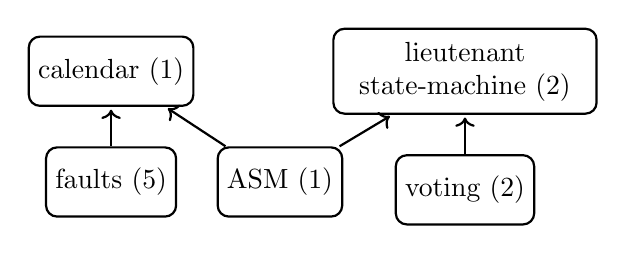
\begin{tikzpicture}[->, node distance=2.6cm, auto, shorten >=1pt, bend angle=45,thick]
    \tikzstyle{every state}=[rectangle, rounded corners]

    \node[state] (calendar) {calendar (1)};
    \node[state] (lieutenant) [right=1.75cm of calendar] {\begin{tabular}{c}lieutenant\\state-machine (2)\end{tabular}};
    \node[state] (faults) [below=0.5cm of calendar] {faults (5)};
    \node[state] (asm) [right=0.5cm of faults] {ASM (1)};
    \node[state] (voting) [below=0.5cm of lieutenant] {voting (2)};

    \tikzstyle{every node}=[]

    \path
    (faults) edge [] node {} (calendar)
    (asm)    edge [] node {} (calendar)
    (asm)    edge [] node {} (lieutenant)
    (voting) edge [] node {} (lieutenant);

  \end{tikzpicture}
  \caption{Invariant classification and dependencies.}
  \label{fig:proof}
\end{figure}

To make the proof scalable, we specify inductive invariants to be used by SAL's $k$-induction engine. There are 11 invariants, falling into five categories:
\begin{enumerate}
  \item \emph{Calendar automata}: Lemmas relating to the calendar automata model. These include lemmas such as time being monotonic, channels missing messages if there is no calendar event, and only nodes associated with a calendar event may execute their local state machines.
  \item \emph{Abstract state machine (ASM)}: Lemmas relating the ASM synchronous observer states to the implementation states.
  \item \emph{Receiver local behavior}: Lemmas describing the modes of behavior of the receivers. The major modes of the state machine are receiving messages, then once it has filled its buffer, it votes, and after voting returns the result. One additional lemma notes that the messages currently received plus missing messages equals the total number of expected messages.
  \item \emph{Faults}: Lemmas characterizing the effect of a fault in a single broadcast. Examples include lemmas stating that if a node receives a faulty message, some ``upstream'' node in the communication path was faulty. Another example is that the faults of messages latched by a node in its buffer match the faults ascribed to the sender in the calendar event.
  \item \emph{Voting}: Lemmas proving that the Fast Majority Vote algorithm implements a majority vote, if one exists. These lemmas are nearly verbatim transcriptions from the journal proofs~\cite{mjrty}.
\end{enumerate}
\noindent
The proof structure is shown in Figure~\ref{fig:proof}. The number of lemmas per category are shown in parentheses. Arrows denote dependencies. For example, the ASM lemmas depend on both the calendar automata and receiver state-machine lemmas. As can be seen, the proof structure is modular. The calendar lemmas are general and independent of any particular protocol or fault model. Similarly, lemmas about the internal behavior of a receiver is independent of the global protocol behavior. It is also independent of the effect of faults on the system---the only ``knowledge'' of faults that receiver has is whether a fault is benign or not. Lemmas about the behavior of faults in the system are also independent of the particular protocol being modeled. Likewise, lemmas about the particular voting algorithm used depend only on the receiver's internal behavior. Only the ASM depends on both calendar-specific and local state-machine results, since it is an abstraction of the entire system implementation. Recall, however, that the ASM is a convenience for debugging and can be elided.

% ------------------------------------------------------------
\section{Experimental Results}\label{sec:experimental}

Here we present two classes of experimental results. First, we demonstrate the scalability results of the verification, despite the low-level modeling. Then we describe modularity results, demonstrated by making modifications to the model and re-validating the model.

\subsection{Scalability}

\begin{figure}
  \centering
  \begin{tabular}{c|c||c|c|c|c|c|c|c|c|c|c|}
      \multicolumn{1}{r}{} & \multicolumn{1}{r}{} & \multicolumn{10}{c}{Receivers} \\
      \cline{2-12}
          &     & 1  &  2  &   3  &  4  &   5  &  6   &  7   &  8  &  9  &  10 \\
      \cline{2-12} \cline{2-12}
          \multirow{10}{*}{Relays\phantom{x}} &
            1   & 7    & 9   & 12   & 15  & 21   & 25   & 32   & 40  & 54  & 74  \\
      \cline{2-12}
          & 2   & 17   & 14  & 21   & 30  & 42   & 53   & 74   & 99  & 144 & -   \\
      \cline{2-12}
          & 3   & 21   & 22  & 40   & 50  & 81   & 102  & 155  & 279 & -   & -   \\
      \cline{2-12}
          & 4   & 27   & 34  & 59   & 99  & 141  & 237  & 1114 & -   & -   & -   \\
      \cline{2-12}
          & 5   & 22   & 94  & 125  & 335 & \TO   & 1406 & -    & -   & -   & -   \\
      \cline{2-12}
          & 6   & 36   & 132 & 2966 & 844 & 2457 & -    & -    & -   & -   & -   \\
      \cline{2-12}
          & 7   & 83   & 487 & \TO   & \TO  & -    & -    & -    & -   & -   & -   \\
      \cline{2-12}
          & 8   & 298  & \TO  & \TO   & -   & -    & -    & -    & -   & -   & -   \\
      \cline{2-12}
          & 9   & 1428 & \TO  & -    & -   & -    & -    & -    & -   & -   & -   \\
      \cline{2-12}
          & 10   & \TO   & -   & -    & -   & -    & -    & -    & -   & -   & -   \\
      \cline{2-12}
  \end{tabular}
  \caption{Benchmark of full proof computation time for $\OMH(1)$ implementation. Times are in seconds with a timeout (\TO) limit of one hour. Dashes ('-') denote no benchmark was run.}
  \label{fig:benchmark}
\end{figure}

We present benchmarks in Figure~\ref{fig:benchmark}. The benchmarks were
performed on a server with Intel Xeon E312xx (Sandy Bridge) CPUs (mid 2011). The table provides execution times in seconds, with a timeout limit of one hour, for verifying the model, given a selected number of relays and receivers. The voting logic is in the receivers, so they have substantially more state than the relays, and dominate the execution time. The execution times sums the execution times for verifying each of the eleven lemmas individually, as well as the final agreement and validity theorems. Each proof incurs the full startup, parsing, type-checking, and model-generation time of SAL. Observe the theorems hold even in the degenerate cases of one relay or one receiver.

As a point of comparison, Rushby presents an elegant model of the simpler \OM{m} algorithm, also in SAL, but using BDD-based model-checking~\cite{Rushby:OM1}. The model is at the algorithmic level. For small values, the verification is much faster, probably due to making only one call to SAL. However, for six relays and two receivers, it takes 449~seconds and timeouts (at one hour) for seven relays and two receivers.

%% For comparison, when the fault model is ``turned off'' by defining the fault
%% type to contain a single 'nonfaulty' value and removing fault specific lemmas,
%% model-checking scales further. For example when there are 3 relays and 3
%% receivers the time is 25s (compared to 40s above), and when where are 5 relays
%% and 5 receivers the time is 315s (compared to timeout above). See Figure
%% \ref{fig:effort} for more comparisons.

%% \lee{discuss results}

\subsection{Modular Verification}\label{sec:modular}

\begin{figure}
  \centering
  \begin{tabular}{|p{3cm}|p{2cm}|p{2cm}|p{2cm}|p{2cm}|}
  \hline
                                  & Transition systems\linebreak (7 total)  &Definitions\linebreak (58 total) & Invariants\linebreak (11 total) & Invariant classes\linebreak (5 total) \\
  \hline \hline
  %% No Fault Model                  & receivers & 8 modified & 2 modified & ASM, faults \\
  %% \hline
  Omissive Asymmetric Faults       & none      & 1 new, 2 modified & 2 modified & faults             \\
  \hline
  Time-Triggered Messaging        & source, relays, receivers, ASM & 3 new & 2 modified, 3 modified & calendar, faults \\
  \hline
  Mid-Value Selection & receivers & 4 new, 3 modified & 2 modified & ASM, voting \\
  \hline
  \end{tabular}
  \caption{Refactoring effort for protocol modifications, measured by which portions of the model have to be modified.}
  \label{fig:effort}
\end{figure}

To demonstrate the modularity of the model and verification approach, in this section, we explore variants to the model and report the effort required to implement the modifications and repair the proofs. The results are summarized in Figure~\ref{fig:effort} and sketched below. In the table, for each modification, we report how much of the model must be modified. We report on four aspects of the system: which transition systems are modified (as described in Section~\ref{sec:sketch}), how many definitions have to be added or modified, the number of invariants that have to be added or modified, and which invariant classes (as defined in Section~\ref{sec:invariants}) those lemmas belong to. We modify the implementation along the axes of faults, time, and local node behavior.

\paragraph{Omissive Asymmetric Faults.}
Removing faults already described by the fault model is easy. Recall that in our model faults do not appear in the system specification and only operate on the calendar. Removing a fault from the system requires only setting the number of a particular kind of faults to zero in the maximum fault assumption.

Adding new kinds of faults requires more work but is still modular. Consider adding \emph{omissive asymmetric faults}, a restriction of Byzantine faults in which a broadcaster either sends the correct value or a benign fault~\cite{omissive}, to the fault model. Doing so requires modifying none of transition systems, because of the synchronous kibitzer. We add a new uninterpreted function definition for omissive asymmetric faults, then modify the type of faults, and their effect on the calendar. Two invariants, both in the class of invariants cover faults, are extended to cover the cases where a sender is omissive asymmetric.

\paragraph{Time-Triggered Messaging.}
A \emph{time-triggered} distributed system is one in which nodes are independently clocked, but clock constraints allow the model to appear as if it is executing synchronously~\cite{kopetz}.

Changing the model to be time-triggered principally requires making the source, relays, and receivers driven explicitly by the passage of time. As well, a ``receive window'' is defined at which messages from non-faulty nodes should be received. Messages received outside the window are marked as coming from manifest-faulty senders. To implement a time-triggered model, we create three definitions; one encodes nondeterministic message delay, and two are small helpers called by invariants. The guards in the relays and receivers are modified to latch messages received outside the specified windows as being manifest faults. Additionally, the ASM definition is modified to track the times in the calendar, not just the messages. Two new calendar invariants are introduced, stating that the calendar messages are either empty, or their time-stamps fall within the respective message windows. Then, three invariants classifying faults are relaxed to allow for the possibility of faulty nodes sending benign messages.

\paragraph{Mid-Value Selection.}
Our $\OMH(1)$ model leverages a majority vote in order to tolerate faults. Another choice for the fault masking algorithm used is mid-value selection. This choice is common in applications involving hardware, signal selection, or cases where information about congruence is useful. To implement mid-value selection in our model, we allow messages sent to take values in $\mathbb{R}$ and the receiver transition system is modified in two ways. First, a second buffer is introduced which will hold the sorted contents of the main buffer once voting has commenced. Second, a mid-value select function is called on the sorted buffer and the result is stored as the receiver's vote. The only invariants needing modification were the ASM definition (to account for the values stored by the new buffer and the relation between it and the main buffer) and the voting invariant.


\subsection{Proof Effort Remarks}

The lemmas described in Section~\ref{sec:invariants} are constructed by-hand and represent multiple days of effort, but that effort includes both model and protocol construction and generalization as well as verification. The counterexamples returned by SAL are very useful for strengthening invariants, but tedious to analyze---a model with five relays and two receivers contains 90 state variables, and there are known counterexamples to models that size~\cite{Lincoln-Rushby}. Once we developed the ASM synchronously-composed observer, the verification effort was sped up considerably.

The invariants and model are surprisingly modular. The modifications we explored took at most hours to develop. Moreover, most of the invariants do not concern the specific protocol modeled at all, and we hypothesize that for completely different protocols, only the modeling aspects related to the protocol behavior and local node behavior would change.

Moreover, we are agnostic about how lemmas are discovered. As techniques like IC3 scale, they may be discovered automatically. $k$-induction in infinite-state model-checking blurs the lines between interactive and automated theorem proving. IC3 can even be strengthened using $k$-induciton~\cite{pdr-kind}. Tools like Ivy can present graphical counterexamples to help interactively develop invariants~\cite{ivy}.

% ------------------------------------------------------------
\section{Related Work}\label{sec:related}

The Oral Messages algorithm and its variants and its variants have a long history of formal verification. \OM{1} was verified in both the PVS and ACL2 interactive theorem-provers~\cite{Young97:IC}. Also in ACL2, an implementation of a circuit design to implement \OM{1} is given~\cite{om-acl2-impl}; the low-level model most closely relates to our level of detail. A refinement-based verification approach is used, and \OM{1} is specialized to a four-node system. It appears that a general purpose voting algorithm (like Fast MJRTY) is not verified as part of the work. It is not clear how difficult it would be to model and verify changes to the implementation in that framework.

Using automated techniques, Gasc{\'{o}}n and Tiwari use SAT-based bounded synthesis to partially synthesize a variant of Oral Messages that tolerates transient faults, specialized for three or four nodes~\cite{om1-synth}. Bokor~\emph{et~al.} describe a message-passing model for synchronous distributed algorithms that is particularly amenable to partial-order reduction for explicit-state model-checking~\cite{Bokor2010}. The model is efficient for up to five nodes, but results are not presented beyond that. Very recently, Jovanovi{\'{c}} and Dutertre use a ``flattened'' high-level model of \OM{1} as a benchmark for IC3 augmented with $k$-induction~\cite{pdr-kind}.

% ------------------------------------------------------------
\section{Conclusions}\label{sec:conclusions}
This work fits within a larger project, in collaboration with Honeywell Labs, to build an \emph{architectural domain-specific language} (ADSL) for specifying and verifying distributed fault-tolerant systems. The goal of the language is to synthesize both software and/or hardware implementations as well as formal models for verification. Before building such an ADSL, we needed a scalable general formal model to which to compile, leading to the work presented in this paper. We hypothesize that an ADSL will make refactoring even easier, and we can generate invariants or invariant templates useful for verification. Indeed, we have developed a preliminary ADSL that generates C code as well as formal models SRI's Sally~\cite{pdr-kind}, to be described in future work.\footnote{\url{https://github.com/GaloisInc/atom-sally}}

Beyond building an ADSL, another avenue of research is producing a formal proof that a software implementation satisfies the node specification in our framework. While our model of node behavior is low-level, there are gaps. For example, our work is in SAL's language of guarded commands~\cite{SAL} and needs to be either refined or verified to be equivalent to a software implementation's semantics. Another aspect is that behavior related to networking and benign fault diagnosis (e.g., computing a CRC) is are left abstract. In a software implementation, the $send$ and $recv$ functions would have to implement these behaviors.



 %% A synthesis approach may be suitable and has been used in the past for fault-tolerant clock-synchronization~\cite{ddd}.



\lee{link to all results in github}
\lee{talk about compositional verification of properties, even though SAL doesn't directly support it---maybe not so important}
\lee{talk about k-induction vs. PDR---actually I don't think we have much to say}
\lee{talk about lack of axiomatization in model-checking (multiple rushby bugs), but  tradeoff of deadlock. see proglema paper}

\section*{Acknowledgments}
This work is partially supported by NASA contract \#NNL14AA08C. We are indebted to our collaborators Brendan Hall and Srivatsan Varadarajan at Honeywell Labs, and to Wilfredo Torres-Pomales at NASA Langley for their discussions and insights. Additionally, we acknowledge that this work is heavily inspired by a series of papers authored by John Rushby.

\bibliographystyle{IEEEtran}
\bibliography{paper}

\end{document}
